\documentclass[theme=teal]{khmermath}

% =========================================================================
% គម្រូឯកសារមេរៀន និងលំហាត់គណិតវិទ្យា (Korean Textbook Style Template)
% =========================================================================

\geometry{left=0.85cm, right=0.85cm, top=0.75cm, bottom=1.5cm, footskip=0.7cm}
\usepackage{colortbl}
\usepackage{tikz}
\usetikzlibrary{calc,shapes,arrows,intersections,through,backgrounds,shadows,decorations.pathmorphing}

% -------------------------------------------------------------------------
% ពណ៌ស្តង់ដារ (Color Palette)
% -------------------------------------------------------------------------
\definecolor{koreaTeal}{RGB}{0, 150, 155}       % ពណ៌ផ្ទៃបដាខាងលើ (Header Teal)
\definecolor{koreaDarkTeal}{RGB}{0, 105, 110}   % ពណ៌ចំណងជើង និងអក្សរសំខាន់
\definecolor{koreaBeige}{RGB}{247, 244, 237}     % ពណ៌ផ្ទៃប្រអប់ (Background Beige)
\definecolor{koreaOrange}{RGB}{235, 115, 30}     % ពណ៌លេខលំហាត់ និង Badge កម្រិតងាយ
\definecolor{koreaBlue}{RGB}{35, 110, 190}      % ពណ៌កម្រិតមធ្យម
\definecolor{koreaPurple}{RGB}{125, 50, 160}    % ពណ៌កម្រិតជឿនលឿន
\definecolor{koreaNumber}{RGB}{115, 125, 135}   % ពណ៌ខ្ទង់ទីមួយនៃលេខលំហាត់
\definecolor{koreaYellow}{RGB}{255, 246, 175}   % ពណ៌ Highlight
\definecolor{brandNavy}{RGB}{0, 105, 110}
\definecolor{brandBlue}{RGB}{0, 150, 155}
\definecolor{brandLightBlue}{RGB}{247, 244, 237}
\definecolor{brandCrimson}{RGB}{195, 35, 60}
\definecolor{brandGold}{RGB}{215, 130, 10}
\definecolor{brandTeal}{RGB}{0, 150, 155}
\definecolor{brandTealBg}{RGB}{244, 252, 250}
\definecolor{cardBorder}{RGB}{220, 212, 198}

% -------------------------------------------------------------------------
% ក្បាលទំព័រ និងជើងទំព័រ (Header & Footer Setup)
% -------------------------------------------------------------------------
\usepackage{fancyhdr}
\pagestyle{fancy}
\fancyhf{}
\renewcommand{\headrulewidth}{0pt}
\renewcommand{\footrule}{\color{koreaTeal!60}\hrule height 0.6pt\vspace{3pt}}

% សូមកែប្រែព័ត៌មានខាងក្រោមតាមតម្រូវការ៖
\newcommand{\LessonNum}{មេរៀនទី ...}
\newcommand{\LessonTitle}{ចំណងជើងមេរៀន}
\newcommand{\TeacherName}{ក្រូត រស្មី}
\newcommand{\ContactPhone}{070897540}

\fancyfoot[L]{%
  \fontsize{8.5}{8.5}\selectfont\kml \color{koreaNumber}\textbf{\thepage}\ \vline\ \color{koreaDarkTeal}\textbf{\LessonTitle}%
}
\fancyfoot[C]{%
  \fontsize{8.5}{8.5}\selectfont\kby \color{koreaDarkTeal}\textbf{\ding{72}\ បង្រៀនដោយ ៖ \textcolor{koreaDarkTeal}{\TeacherName}\ \ding{72}}%
}
\fancyfoot[R]{%
  \fontsize{8.5}{8.5}\selectfont\kby \color{koreaDarkTeal}\textbf{ Telegram: \textcolor{brandCrimson}{\ContactPhone}}\ \vline\ \color{koreaNumber}\textbf{\thepage}%
}

% -------------------------------------------------------------------------
% បដាចំណងជើងធំ (Korean Header Banner)
% -------------------------------------------------------------------------
\newcommand{\koreanheader}[2]{%
  \noindent%
  \begin{tikzpicture}[x=1cm, y=1cm]
    \fill[koreaTeal, rounded corners=12pt] (0, 0.1) -- (0, 0.95) -- (3.8, 0.95) [rounded corners=0pt] -- (4.4, 0.1) -- cycle;
    \node[white, font=\fontsize{11}{11}\selectfont\kml\bfseries] at (1.9, 0.52) {#1};
    \node[anchor=west, font=\fontsize{18}{18}\selectfont\kml\bfseries, color=koreaDarkTeal] at (4.6, 0.42) {#2};
    \node[anchor=east, font=\fontsize{8.5}{8.5}\selectfont\kby, color=gray!80] at (19.2, 0.48) {$>$ ក្លឹបសិក្សាគណិតវិទ្យា ភី ស៊ី​ អឹម};
  \end{tikzpicture}%
  \vspace{3pt}%
}

% -------------------------------------------------------------------------
% សញ្ញាសម្គាល់កម្រិត និងអក្សរ (Badges)
% -------------------------------------------------------------------------
\newcommand{\badgebasic}{\tikz[baseline=(char.base)]{\node[rounded corners=3.5pt, fill=koreaOrange, text=white, font=\fontsize{8.5}{8.5}\selectfont\kml\bfseries, inner sep=2.5pt] (char) {\ding{72}\ គ្រឹះ};}}
\newcommand{\badgestandard}{\tikz[baseline=(char.base)]{\node[rounded corners=3.5pt, fill=koreaTeal, text=white, font=\fontsize{8.5}{8.5}\selectfont\kml\bfseries, inner sep=2.5pt] (char) {\ding{72}\ding{72}\ មធ្យម};}}
\newcommand{\badgeadvanced}{\tikz[baseline=(char.base)]{\node[rounded corners=3.5pt, fill=koreaPurple, text=white, font=\fontsize{8.5}{8.5}\selectfont\kml\bfseries, inner sep=2.5pt] (char) {\ding{72}\ding{72}\ding{72}\ ជឿនលឿន};}}
\newcommand{\secbadge}[1]{\tikz[baseline=(char.base)]{\node[circle, fill=brandNavy, inner sep=2.5pt, text=white, font=\fontsize{8.5}{8.5}\selectfont\bfseries] (char) {#1};}}
\newcommand{\alphabadge}[1]{\tikz[baseline=(char.base)]{\node[fill=brandCrimson, text=white, rounded corners=4pt, minimum size=15pt, inner sep=1pt, align=center, font=\fontsize{8.5}{8.5}\selectfont\bfseries] (char) {#1};}}

% -------------------------------------------------------------------------
% ប្រអប់ទ្រឹស្តី និងកាត (Styled Boxes)
% -------------------------------------------------------------------------
% ប្រអប់ទ្រឹស្តីទូទៅ (General Box)
\newtcolorbox{khboxorange}[1][]{
  enhanced,
  colframe=brandNavy!40,
  colback=brandLightBlue,
  boxrule=0.7pt,
  arc=5.0pt,
  borderline west={3.5pt}{0pt}{brandNavy},
  drop fuzzy shadow=brandNavy!15,
  left=10pt, right=10pt, top=7pt, bottom=6pt,
  title={\fontsize{9.5}{9.5}\selectfont\kml\color{white}\ding{72}\ ជាទូទៅ},
  coltitle=white,
  colbacktitle=brandNavy,
  boxed title style={
    boxrule=0pt,
    arc=3.5pt,
    left=7pt, right=7pt, top=2.5pt, bottom=2.5pt
  },
  attach boxed title to top left={yshift*=-\tcboxedtitleheight/2, xshift=12pt},
  #1
}

% កាតសង្ខេបចំណុច (Card Item Box)
\newtcolorbox{khcard}[1][]{
  enhanced,
  colframe=cardBorder,
  colback=white,
  boxrule=0.7pt,
  arc=3.5pt,
  left=6pt, right=6pt, top=4pt, bottom=4pt,
  #1
}

% -------------------------------------------------------------------------
% ចំណងជើងផ្នែកធំ និងផ្នែករង (Section & Subsection Banners)
% -------------------------------------------------------------------------
\newcommand{\khsection}[2]{%
  \vspace{6pt}%
  \noindent%
  \begin{tikzpicture}
    \fill[rounded corners=5pt, brandNavy!7] (0,0) rectangle (19.3, 0.72);
    \fill[rounded corners=4pt, brandNavy] (0.06, 0.06) rectangle (0.64, 0.66);
    \node[white, font=\fontsize{10}{10}\selectfont\bfseries] at (0.35, 0.36) {#1};
    \fill[brandGold, rounded corners=1pt] (0.74, 0.16) rectangle (0.78, 0.56);
    \node[anchor=west, font=\fontsize{11.5}{11.5}\selectfont\kml, color=brandCrimson] at (0.85, 0.36) {\textbf{#2}};
  \end{tikzpicture}%
  \vspace{3pt}%
}

\newcommand{\khsubsection}[2]{%
  \vspace{4pt}%
  \noindent%
  \begin{tikzpicture}[baseline=(sub.base)]
    \node[rounded corners=3.5pt, fill=brandBlue!12, draw=brandBlue!35, line width=0.5pt, text=brandNavy, font=\fontsize{9.5}{9.5}\selectfont\kml\bfseries, inner sep=3.5pt] (sub) at (0,0) {#1};
    \node[anchor=west, font=\fontsize{10.5}{10.5}\selectfont\kml\bfseries, color=brandNavy] at (sub.east) {\ \ #2};
  \end{tikzpicture}%
  \vspace{3pt}%
}

% -------------------------------------------------------------------------
% លេខរៀងលំហាត់រចនាប័ទ្មកូរ៉េ (Two-Tone Exercise Numbering)
% -------------------------------------------------------------------------
\def\splitnum#1#2{%
  \color{koreaNumber!65}#1\color{koreaOrange}#2%
}
\newcommand{\koreannum}[1]{%
  \ifstrempty{#1}{}{%
    \mbox{%
      \fontsize{25}{25}\selectfont\bfseries%
      \ifnum\number#1<10\relax%
        \color{koreaNumber!65}0\color{koreaOrange}\number#1%
      \else%
        \expandafter\splitnum\number#1%
      \fi%
    }\,\ %
  }%
}
\newcommand{\exhead}[1]{\hangindent=26pt\hangafter=1\koreannum{#1}}

\setlength{\parindent}{0pt}
\setlength{\parskip}{3.5pt}

% =========================================================================
% ចាប់ផ្តើមតួខ្លឹមសារឯកសារ (DOCUMENT CONTENT)
% =========================================================================
\begin{document}

% ១. បដាក្បាលទំព័រមេរៀន
\koreanheader{\LessonNum}{\LessonTitle}

\vspace{3pt}
% ២. ចំណងជើងផ្នែកធំទី ១
\khsection{១}{ចំណងជើងផ្នែកធំទីមួយ}

% ផ្នែករង ១.១
\khsubsection{១.១}{ចំណងជើងផ្នែករង}

% ប្រអប់ទ្រឹស្តី ឬរូបមន្តគន្លឹះ
\begin{khboxorange}
  \begin{itemize}[leftmargin=15pt, itemsep=2pt, topsep=1pt, parsep=0pt]
    \item[\color{brandNavy}\ding{228}] \textbf{ទ្រឹស្តីបទ ឬរូបមន្តគន្លឹះសំខាន់ទី ១ ៖ សរសេរខ្លឹមសារនៅទីនេះ ។}
    \item[\color{brandNavy}\ding{228}] \textbf{ទ្រឹស្តីបទ ឬរូបមន្តគន្លឹះសំខាន់ទី ២ ៖ សរសេរខ្លឹមសារនៅទីនេះ ។}
  \end{itemize}
\end{khboxorange}

\vspace{3pt}

% ៣. ផ្នែកលំហាត់ (រៀបជា ២ ជួរ ដោយមានបន្ទាត់ពុះកណ្តាល)
\setlength{\columnsep}{18pt}
\setlength{\columnseprule}{0.5pt}
\def\columnseprulecolor{\color{cardBorder}}

\begin{multicols}{2}
  % ----------------- ជួរទី ១ (Column 1) -----------------
  % លំហាត់ ០១ (សរសេរ \exhead{1} វានឹងបង្ហាញជា 01 ពីរខ្ទង់ស្វ័យប្រវត្តិ)
  \noindent
  \exhead{1} គេមានត្រីកោណ $ABC$ កែងត្រង់ $A$ ដែលមានជ្រុង $AB = 6\text{cm}$ និង $AC = 8\text{cm}$ ៖ គណនាប្រវែងអ៊ីប៉ូតេនុស $BC$ ៖\par
  \vspace{2pt}
  {\centering
    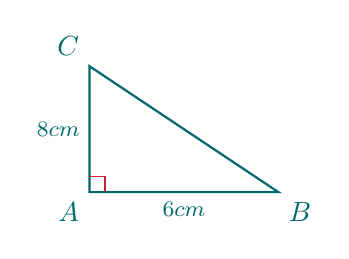
\begin{tikzpicture}[scale=0.8]
      \coordinate (A) at (0,0);
      \coordinate (B) at (3,0);
      \coordinate (C) at (0,2);
      \draw[thick, color=brandNavy] (A) node[below left] {$A$} -- (B) node[below right] {$B$} -- (C) node[above left] {$C$} -- cycle;
      \draw[color=brandCrimson, line width=0.5pt] (0, 0.25) -- (0.25, 0.25) -- (0.25, 0);
      \node[below, color=brandNavy] at (1.5, 0) {\footnotesize $6\text{cm}$};
      \node[left, color=brandNavy] at (0, 1) {\footnotesize $8\text{cm}$};
    \end{tikzpicture}\par}

  \vspace{5pt}
  % លំហាត់ ០២
  \noindent
  \exhead{2} រកតម្លៃនៃ $x$ ក្នុងរូបខាងក្រោម ៖\par
  \begin{itemize}[leftmargin=15pt, itemsep=2pt, topsep=1pt]
    \item[\alphabadge{ក}] រកប្រវែងជ្រុង $AB$
    \item[\alphabadge{ខ}] រកតម្លៃ $x$
  \end{itemize}

  \columnbreak

  % ----------------- ជួរទី ២ (Column 2) -----------------
  % លំហាត់ ០៣
  \noindent
  \exhead{3} គណនាក្រឡាផ្ទៃ និងបរិមាត្រនៃរង្វង់ដែលមានកាំ $r = 7\text{cm}$ ដោយយក $\pi \approx \frac{22}{7}$ ៖\par
  \vspace{2pt}
  {\centering
    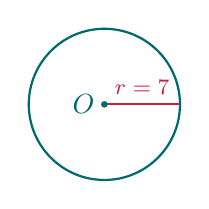
\begin{tikzpicture}[scale=0.8]
      \draw[thick, color=brandNavy] (0,0) circle (1.2);
      \coordinate (O) at (0,0);
      \coordinate (R) at (1.2,0);
      \draw[thick, color=brandCrimson] (O) -- (R) node[midway, above] {\footnotesize $r = 7$};
      \fill[brandNavy] (O) circle (1.5pt) node[left] {$O$};
    \end{tikzpicture}\par}

  \vspace{5pt}
  % លំហាត់ ០៤
  \noindent
  \exhead{4} ចូរដោះស្រាយសមីការខាងក្រោម ៖
  \begin{itemize}[leftmargin=15pt, itemsep=2pt, topsep=1pt]
    \item[\alphabadge{ក}] $2x + 5 = 15$
    \item[\alphabadge{ខ}] $3(x - 2) = 2x + 4$
  \end{itemize}
\end{multicols}

\vspace{6pt}

% ៤. បដាពាក្យស្លោកខាងក្រោម (Bottom Motto Banner)
\begin{tcolorbox}[
  enhanced,
  colback=brandTealBg,
  colframe=brandNavy!30,
  arc=3pt,
  boxrule=0.6pt,
  top=2.5pt, bottom=2.5pt,
  center,
  halign=center
]
  \fontsize{9}{9}\selectfont\kml\color{brandNavy}
  \textbf{\ding{228}\ ខំរៀនដើម្បីខ្លួនឯង និងអនាគតដ៏ភ្លឺស្វាង \ding{228}}
\end{tcolorbox}

\end{document}
